\documentclass[12pt]{article}
\usepackage[margin=1in]{geometry}
\usepackage{graphicx}
\usepackage{float}
\usepackage{hyperref}
\usepackage{amssymb}
\usepackage{amsmath}
\usepackage[]{algorithm2e}
\usepackage{fancyhdr}

\pagestyle{fancy}
\fancyhf{}
\rhead{Mucong Ding}
\lhead{mcding@mit.edu}

\begin{document}

\title{Answer to 6.437 Project Part I}

\author{Mucong Ding, mcding@mit.edu, Stu ID: 920494196}

\maketitle

\section{Problem 1}
\subsection{(a)}
Since we assume English text can be modeled as a Markov chain, the probability of a plaintext $\mathbf{x}$ is:
\begin{equation}
\begin{split}
	p_{\mathbf{x}}(\mathbf{x}) & = \mathbb{P}(x_1)\mathbb{P}(x_2|x_1)\cdots\mathbb{P}(x_n|x_{n-1})\\ 
	& = P_{x_1}\Pi_{i=2}^{n-1}M_{x_{i+1},x_i}
\end{split}
\end{equation}
Thus the probability of corresponding ciphertext $\mathbf{y}$ encrypted by cipher function $f$ is:
\begin{equation}
\label{likelihood}
	p_{\mathbf{y}|f}(\mathbf{y}|f) = P_{f^{-1}(y_1)}\Pi_{i=2}^{n-1}M_{f^{-1}(y_{i+1}),f^{-1}(y_i)}
\end{equation}
And this is the likelihood of the observed ciphertext $\mathrm{y}$ under ciphering function $f$.

\subsection{(b)}
By Bayes' rule, the posterior distribution is simply:
\begin{equation}
	p_{f|\mathbf{y}}(f|\mathbf{y}) = \frac{p_{\mathbf{y}|f}(\mathbf{y}|f)p_{f}(f)}{\Sigma_{f}p_{\mathbf{y}|f}(\mathbf{y}|f)p_{f}(f)}
\end{equation}
Since we adopt a uniform prior:
\begin{equation}
	p_{f}(f) = \frac{1}{|\mathcal{F}|}
\end{equation}
where $\mathcal{F}$ is the set of all possible cyphering functions (permutations on $\mathcal{A}$, $\mathcal{F}=\text{Perm}(\mathcal{A})$). We can simplify the formula of $p_{f|\mathbf{y}}(f|\mathbf{y})$ to:
\begin{equation}
p_{f|\mathbf{y}}(f|\mathbf{y}) = \frac{p_{\mathbf{y}|f}(\mathbf{y}|f)}{\Sigma_{f}p_{\mathbf{y}|f}(\mathbf{y}|f)}
\end{equation}
And the MAP estimator $\hat{f}_{\text{MAP}}(\mathbf{y})$ is:
\begin{equation}
	\hat{f}_{\text{MAP}}(\mathbf{y}) = \arg\max_{f}p_{f|\mathbf{y}}(f|\mathbf{y})
\end{equation}
Again because we assume uniform prior, it could be simplify to:
\begin{equation}
\begin{split}
	\hat{f}_{\text{MAP}}(\mathbf{y}) & = \arg\max_{f}p_{\mathbf{y}|f}(\mathbf{y}|f) \\ & = \arg\max_{f}P_{f^{-1}(y_1)}\Pi_{i=2}^{n-1}M_{f^{-1}(y_{i+1}),f^{-1}(y_i)}
\end{split}
\end{equation}
It's the same as the ML estimator.

\subsection{(c)}
Direct evaluation of the MAP estimate $\hat{f}_{\text{MAP}}$ is computationally infeasible since the alphabet of ciphering functions, $\mathcal{F}$, is too large:
\begin{equation}
	|\mathcal{F}| = |\mathcal{A}|! = 28! = 304888344611713860501504000000
\end{equation}
It's infeasible to iterate through this alphabet to find $\hat{f}_{\text{MAP}}$ which maximizes $p_{f|\mathbf{y}}(f|\mathbf{y})$.


\section{Problem 2}
\subsection{(a)}
Fist note that for each specific ciphering function $f$ (permutation on $\mathcal{A}$), it has ${|\mathcal{A}|\choose2}$ "neighbors" which differ in exactly two symbol assignments. Thus, since there are $|\mathcal{F}| = |\mathcal{A}|!$ cipher functions, there are:
\begin{equation}
	\frac{|\mathcal{A}|!}{2}{|\mathcal{A}|\choose2}
\end{equation}
such "neighboring" pairs. And since there are ${|\mathcal{A}|!\choose2}$ cipher function pairs, and we assume they are uniformly distributed. The probability that a pair of ciphering functions $f_1$ and $f_2$ differ in exactly two symbol assignments is:
\begin{equation}
\begin{split}
	\mathbb{P}&(\text{"pair differ  exactly two assigments"}) = \frac{\frac{|\mathcal{A}|!}{2}{|\mathcal{A}|\choose2}}{{|\mathcal{A}|!\choose2}} \\ & = \frac{378}{28!-1} \approx 1.2397981\times{10}^{-27}
\end{split}
\end{equation}

\subsection{(b)}
Inspired by problem 2(a), we construct the proposal transition matrix as:
\begin{equation}
V(f'|f) =
\begin{cases}
\frac{1}{{28\choose2}} & \text{if } f'\in \text{Nei}(f) \\
0 & \text{elsewise}
\end{cases}
\end{equation}
where $\text{Nei}(f)$ is the set of permutations which differs to $f$ in exactly two symbol assignments.

Following the Metropolis-Hastings algorithm, the effective transition matrix is:
\begin{equation}
	W(f'|f) = V(f'|f)a(f\to f')\quad\text{if }f'\in \text{Nei}(f)
\end{equation}
where $a(f\to f') = \min\big\{1, \frac{p_{\mathbf{y}|f}(\mathbf{y}|f')}{p_{\mathbf{y}|f}(\mathbf{y}|f)}\big\}$ and the likelihood function $p_{\mathbf{y}|f}(\mathbf{y}|f)$ is understand as the "un-normalized" posterior.

By the normalization constraints, the full formula of the effective transition matrix $W$ is:
\begin{equation}
W(f'|f) =
\begin{cases}
\frac{1}{378}\min\big\{1, \frac{p_{\mathbf{y}|f}(\mathbf{y}|f')}{p_{\mathbf{y}|f}(\mathbf{y}|f)}\big\} & \text{if }f'\in \text{Nei}(f)\\ 1-\Sigma_{f'\in\text{Nei}(f)}W(f'|f) & \text{if }f'=f\\0 & \text{elsewise}
\end{cases}
\end{equation}
This defines a Markov chain whose stationary distribution is the posterior $p_{f|\mathbf{y}}(f|\mathbf{y})$.

\subsection{(c)}
Pseudo-code of Metropolis-Hastings algorithm for decoding the ciphertext:

\begin{algorithm}[H]
	\KwIn{alphabet $\mathcal{A}$, ciphertext $\mathbf{y}$, maximum number of iterations $T_\text{max}$, termination threshold $T_\text{term}$}
	\KwResult{predicted cipher function $f_\text{pred}$}
	Initialization: randomly pick $f\in \text{Perm}(\mathcal{A})$\;
	$t=0$, $t_{\text{fixed}}=0$\;
	\While{$t_\text{fixed}<T_\text{term}$ and $t<T_\text{max}$}{
		Get $f'$ by randomly swap two mapped values in $f$\;
		Calculate the likelihoods $p_{\mathbf{y}|f}(\mathbf{y}|f')$ and $p_{\mathbf{y}|f}(\mathbf{y}|f)$ by Eq. \ref{likelihood}\;
		\If{$p_{\mathbf{y}|f}(\mathbf{y}|f')>p_{\mathbf{y}|f}(\mathbf{y}|f)$}{
			f = f'\;
		}\Else{
			Generate random number $x\in[0,1]$\;
			\If{$x<p_{\mathbf{y}|f}(\mathbf{y}|f')/p_{\mathbf{y}|f}(\mathbf{y}|f)$}{
				f = f'\;
			}\Else{
				$t_{\text{fixed}} += 1$\;
			}
		}
		$t+=1$\;
	}
	$f_{\text{pred}} = f$\;
\caption{MH decoding algorithm}
\end{algorithm}

The algorithm terminates when either the number of iterations exceed $T_\text{max}$ or the current cipher function $f$ is not updated for $T_\text{term}$ iterations.


\section{Problem 3}
\subsection{(a)}
The log-likelihood of the accepted state versus iteration count is plotted as Fig. \ref{fig:log-likelihood}. This is the result of one single experiment on the full ciphertext. The x-axis range of the upper plot is $1\leq\text{iter}\leq3000$ and the range of lower plot is $1000\leq\text{iter}\leq3000$.
\begin{figure}[H]
	\centering
	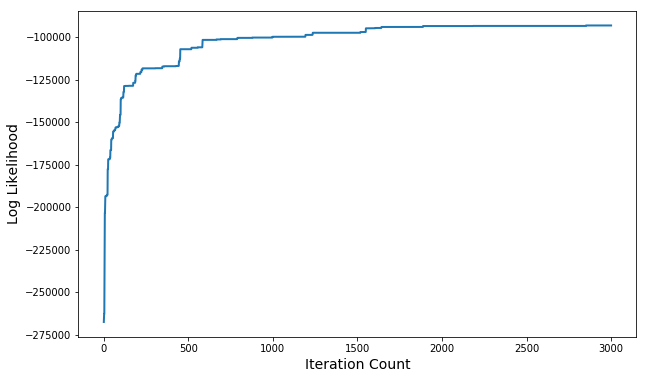
\includegraphics[width=0.9\linewidth]{pics/log-likelihood-1.png}
	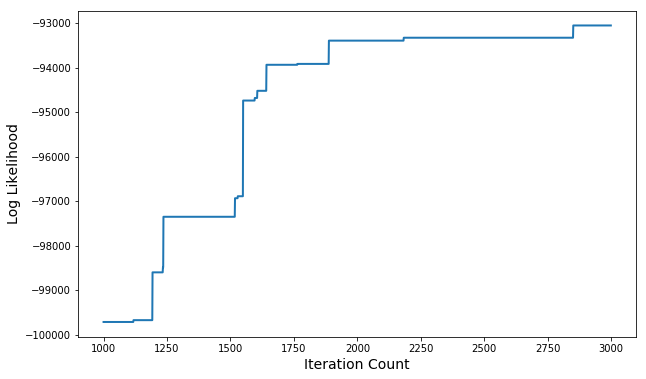
\includegraphics[width=0.9\linewidth]{pics/log-likelihood-2.png}
	\caption{Log-likelihood of the accepted state versus iteration count.}
	\label{fig:log-likelihood}
\end{figure}
We can see the log-likelihood of accepted state is monotonically increasing along with iteration count, and the increasing rate is much larger when the algorithm just starts.

\subsection{(b)}
The acceptance rate of state transitions versus iteration count is plotted as Fig. \ref{fig:acceptance-rate}. Note that the acceptance rate is a sliding window average with window length $T=100$. This is the result of one single experiment on the full ciphertext. The range of x-axis in Fig. \ref{fig:acceptance-rate} is $100\leq\text{iter}\leq3000$.  
\begin{figure}[H]
	\centering
	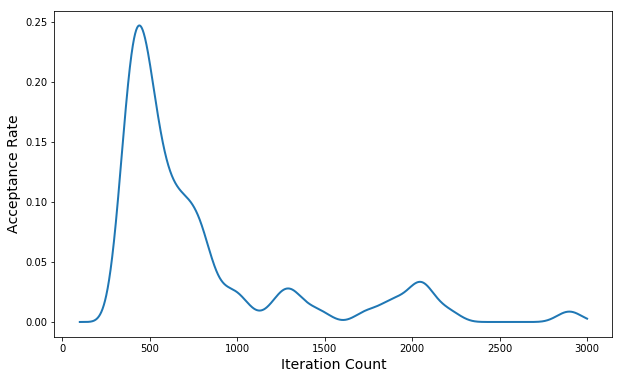
\includegraphics[width=0.9\linewidth]{pics/acceptance-rate.png}
	\caption{Acceptance rate of state transitions versus iteration count.}
	\label{fig:acceptance-rate}
\end{figure}
We can see the acceptance rate first increase rapidly and the drop rapidly. The curve of acceptance rate has a sharp peak at around $\text{iter}\approx400$.

\subsection{(c)}
The accuracy rate versus iteration count is plotted as Fig. \ref{fig:accuracy}. This is the result of one single experiment on the full ciphertext. 
\begin{figure}[H]
	\centering
	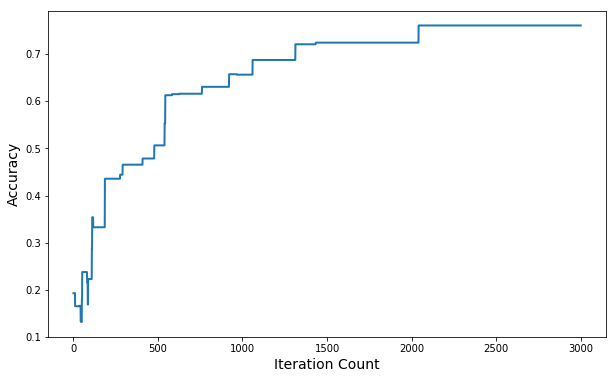
\includegraphics[width=0.9\linewidth]{pics/accuracy.png}
	\caption{Accuracy rate versus iteration count.}
	\label{fig:accuracy}
\end{figure}
We can see the accuracy increase monotonically along with the iteration count. After each increment, there is a plateau. Since it is likely that no updates of the predicted cipher function will take place (because of low acceptance rate) shortly after an update. The terminating accuracy is around $0.78$, which is plausible.

\subsection{(d)}
I run the MCMC-based decoding algorithm on ciphertext with different lengths, ($\text{length}=50, 100, 200, 400, 800, 1600, 3200$) independently. For each ciphertext, I run 20 independent trials and record the average accuracy of the 20 predictions. The average accuracies versus iteration count is plotted as Fig. \ref{fig:text-length}.
\begin{figure}[H]
	\centering
	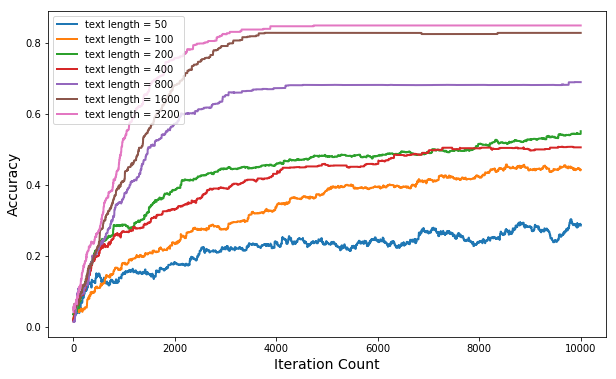
\includegraphics[width=0.9\linewidth]{pics/text-length.png}
	\caption{Average accuracies for ciphertexts of different lengths versus iteration count.}
	\label{fig:text-length}
\end{figure}
We can see that the average accuracies of longer ciphertext strictly bound the average accuracies when predicting on shorter ciphertext. In other word, with the same number of iterations, the average accuracy is monotonically increasing along with the length of input ciphertext. This is because when the input ciphertext is longer, the relative ratio of likelihoods of different cipher functions will be larger or smaller (far away from $1$). In this sense, the MH algorithm will converge faster and achieve a higher accuracy within the same number of iterations.

\subsection{(e)}
I run the MCMC-based decoding algorithm on ciphertext with different lengths, ($\text{length}= 100, 200, 400, 800, 1600$) independently. For each ciphertext, I run 20 independent trials and record the average log-likelihood per symbol (in bits) of the 20 predictions. The average log-likelihood per symbol (in bits) versus iteration count is plotted as Fig. \ref{fig:text-length}. The two plots are the same set of curves with different x-axis range. The x-axis range of the upper plot is $1\leq\text{iter}\leq5000$, and is $1000\leq\text{iter}\leq5000$ for the lower one. 
\begin{figure}[H]
	\centering
	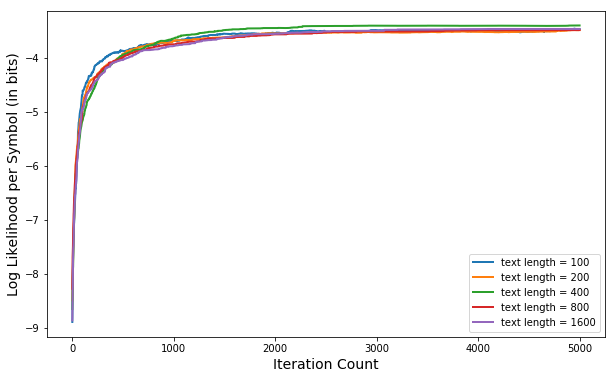
\includegraphics[width=0.9\linewidth]{pics/entropy-1.png}
	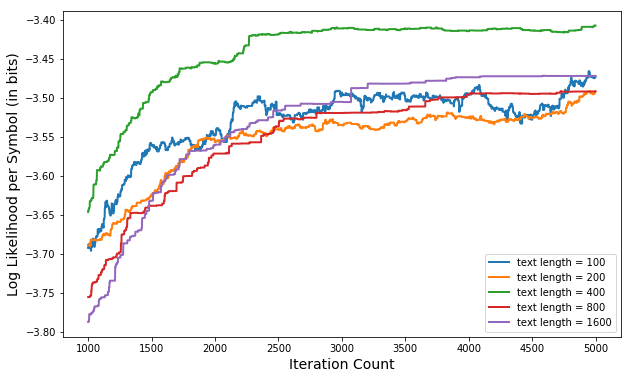
\includegraphics[width=0.9\linewidth]{pics/entropy-2.png}
	\caption{Average log-likelihood per symbol (in bits) versus iteration count.}
	\label{fig:entropy}
\end{figure}
We can see that the steady state values of these curves are generally independent of the length of ciphertext used. And this average is around $-3.50$. Since the steady state distribution of our MCMC-based algorithm is just the distribution of English texts (modeled as Markov chains), we can say that the steady value of these curves, $-3.50$, is the expectation value of the log-likelihood per symbol for English text. And clearly it is just the negative average Entropy per English symbol. From this, we can say the average entropy of English text is roughly $3.50$ bits per symbol (letter). This empirical estimation is slightly larger than Shannon's estimation in "Prediction and Entropy of Printed English", which is $2.3$ bits instead. But at least their magnitudes are similar, and this small difference is reasonable since the empirical entropy of English text depends on how the alphabet is modeled.
\end{document}
